\documentclass[10pt,twoside,a4paper]{article}
\usepackage{etex}
\reserveinserts{28}

\usepackage{polski}
\usepackage[utf8]{inputenc}
\usepackage{pdfpages} % \includepdf
\usepackage{tabu} % \tabu

\usepackage[T1]{fontenc}
\usepackage{uarial}
\renewcommand{\familydefault}{\sfdefault}

\usepackage{geometry}                 % do marginesow
\usepackage{indentfirst}              % zeby pierwsze akapity tez mialy wciecie
\usepackage{titlesec}                 % żeby formatować tytuły rozdziałów itd.
\usepackage{secdot}                   % aby dodać kropkę za numerkiem podrzodziałów i podpodrozdziałów
\usepackage{chngcntr}                 % umożliwia numerowanie obrazków itp. względem rozdziału
\usepackage{tocloft}                  % umożliwia ustawienia dotyczące spisu treści i innych spisów
\usepackage{tabu}                     % do tabel
%\usepackage[table]{xcolor}            % do kolorowania tabel
\usepackage{tabularx}                 % do lepszych tabel
\usepackage[backend=bibtex, language=polish]{biblatex} % do bibliografii
\usepackage{enumitem}                 % do modyfikacji listy (begin{itemize}, niepotrzebne odstępy przed i po)
\usepackage{floatrow}                 % aby umożliwić wymuszenie położenia figury
\usepackage{caption}                  % do zmiany podpisów tabel i obrazków
\usepackage{setspace}                 % również do zmiany podpisów (konkretniej interlinii w podpisach - wymagany przez caption)
\usepackage{longtable}
\usepackage{booktabs}

\usepackage{amsthm}
\usepackage{amsfonts}
\usepackage{hyperref}
\usepackage{physics}
\usepackage{listings}

\newtheorem{placeholder}{PLACEHOLDER}

\newtheorem{definition}[placeholder]{Definicja}
\newtheorem{theorem}[placeholder]{Twierdzenie}
\newtheorem{example}[placeholder]{Przykład}
\newtheorem{remark}[placeholder]{Uwaga}
\newtheorem{corollary}[placeholder]{Wniosek}
\newtheorem{fact}[placeholder]{Fakt}
\newtheorem{convention}[placeholder]{Umowa}


% to jest jakas magia, aby odczytac szerokość longtable i ustawić tę wartość później jako LTcapwidth (parametr kontrolujący szerokość captiona w longtable)
% Creditsy i flaszkę proszę wysyłać do magika Heiko (http://compgroups.net/comp.text.tex/longtable-tablewidth/1922986)
\makeatletter
\newlength\LongtableWidth
\newcommand*{\org@longtable}{}
\let\org@longtable\longtable
\def\longtable{
  \begingroup
    \advance\c@LT@tables\@ne
    \edef\x{LT@\romannumeral\c@LT@tables}
    \global\LongtableWidth\z@
    \@ifundefined{\x}{
      % longtable width not available
    }{
      \def\LT@entry##1##2{
        \global\advance\LongtableWidth##2\relax
      }
      \@nameuse{\x}
    }
    % debug output
    \typeout{* \x: \the\LongtableWidth}
  \endgroup
  \ifdim\LongtableWidth>\z@
    \setlength{\LTcapwidth}{\LongtableWidth}
  \fi
  \org@longtable
}
\makeatother

% Rozpocznij od nowa numerowanie rysunków dla każdego rozdziału (section).
% Dodaje numer rozdziału do numeru rysunku: nr_rozdzial.nr_rysunku_w_ramach_rozdzialu
%
% Źródło: http://tex.stackexchange.com/questions/28333/continuous-v-per-chapter-section-numbering-of-figures-tables-and-other-docume
\counterwithin{figure}{section}

% to samo dla tabel
\counterwithin{table}{section}

% żeby nie było Rysunek tylko Rys
\renewcommand{\figurename}{Rys.}

% żeby nie było odstępów przed/po/w środku listy (itemize, ew. dodać też dla enumerate?)
\setlist[itemize]{noitemsep,nolistsep,topsep=0pt}

% ustawiamy domyślny odstęp przed i po pływającymi elementami (tabele i obrazki) umieszczonymi w środku tekstu (flaga H) na 0
\setlength{\intextsep}{0mm}
\setlength{\textfloatsep}{0mm}

% ustawiamy domyślną czcionkę dla podpisów na small (9pt dla article 10pt) oraz interlinię na 1.0
\captionsetup{font={small,stretch=1.0}}

% własny separator do podpisów (to, co jest po 'Rys. X.Y' - kropka, nazwana wewnętrznie jako 'dot')
\DeclareCaptionLabelSeparator{dot}{. }
\DeclareFloatVCode{6ptskip}{\vspace{6pt}}
\DeclareFloatVCode{12ptskip}{\vspace{12pt}}

% dla tabel: 0pt pod opisem, 6pt nad
\captionsetup[table]{singlelinecheck=false} % nie wyśrodkowywuj opisu w pojedynczej linii
\captionsetup[table]{labelfont=bf,labelsep=dot} % pogrubienie nagłówka podpisu (Tabela X.Y) i zakonczenie jej wczesniej zdefiniowana kropką
\floatsetup[table]{font={small,stretch=1.0},capposition=top,captionskip=0pt,precode=12ptskip,postcode=12ptskip} % nie wiem dlaczego, aby otrzymac odstep 6pt przed tabela, trzeba tutaj dac 12pt :/

\setlength{\LTpre}{12pt}
\setlength{\LTpost}{12pt}

\tabulinesep=2.0mm % wzięte z czapy, ale wygląda dobrze (minimalny odstęp między początkkiem i końcem wierwsza a jego zawartością - przydaje się w przypadku zawijanych wierszy)

% dla obrazków: 6pt nad opisem, 12pt pod
\captionsetup[figure]{justification=centering} % inaczej niz w tabelach - zawsze centruj podpis
\captionsetup[figure]{labelsep=dot} % użyj kropki jako separatora ale nie pogrubiaj
\floatsetup[figure]{capposition=bottom,captionskip=6pt,precode=12ptskip,postcode=12ptskip}

% koment do poniższych: bfseries oznacza pogrubienie, itshape kursywę, mdseries normalną
% large = 12pt, small = 9pt (zależne od ustawionego u góry podstawowego 10pt),
% normalsize podstawowy rozmiar czyli 10pt

% formatowanie tytułów rozdziałów (tutaj nazwane sekcjami)
\titleformat{\section}[block]
    {\large\bfseries}           % czcionka ogólna,
    {\thesection .}             % przedrosetek (kropka bo musi mieć kropkę po numerku
    {0.5em}                     % odstęp między przedrostkiem i treścią tytułu
    {\MakeUppercase}            % formatowanie tytułu (chyba bez przedrostka)

% formatowanie tytulow podrozdzialow (tutaj nazwane podsekcjami)
\titleformat*{\subsection}{\normalsize\bfseries\itshape}
\sectiondot{subsection}

% formatowanie tytulow, punktow, podrozdzialow (tutaj nazwane podpodsekcjami)
\titleformat*{\subsubsection}{\normalsize\itshape}
\sectiondot{subsubsection}

\titlespacing*{\section}{0pt}{12pt}{6pt}
\titlespacing*{\subsection}{0pt}{12pt}{6pt}
\titlespacing*{\subsubsection}{0pt}{12pt}{6pt}

% SPIS TRESCI

% zeby w spisie tresci byly tez kropki po numerkach rozdzialow i podrozdzialow itd.
\renewcommand{\cftsecaftersnum}{.}
\renewcommand{\cftsubsecaftersnum}{.}
\renewcommand{\cftsubsubsecaftersnum}{.}
% zeby napis SPIS TRESCI był wielkimi literami, pogrubiony itd
\renewcommand{\cfttoctitlefont}{\normalfont\large\bfseries\MakeUppercase}
% zeby tytuly rozdzialow w spisie oraz numery stron nie byly pogrubione
\renewcommand\cftsecfont{\normalfont}
\renewcommand\cftsecpagefont{\normalfont}
% zeby dla rozdzialow tez byly kropki od napisu do numeru strony
\renewcommand\cftsecleader{\cftdotfill{\cftdotsep}}
% odstepy między akapitami 6pt
\setlength\cftbeforesecskip{6pt}
\setlength\cftbeforesubsecskip{6pt}
% zeby kropki od napisu do numeru strony byly gestsze
\renewcommand{\cftdotsep}{0}

% SPISY

% zmiana nazwy, czcionki, marginesu i separatora dla listy figur
\renewcommand{\listfigurename}{Wykaz rysunków}
\renewcommand{\cftloftitlefont}{\normalfont\large\bfseries\MakeUppercase}
\setlength\cftbeforefigskip{6pt}
\renewcommand{\cftfigaftersnum}{.}

% zmiana nazwa, czcionki, marginesu i separatora dla listy tabel
\renewcommand{\listtablename}{Wykaz tabel}
\renewcommand{\cftlottitlefont}{\normalfont\large\bfseries\MakeUppercase}
\setlength\cftbeforetabskip{6pt}
\renewcommand{\cfttabaftersnum}{.}

% ustawienie marginesow
\geometry{
   a4paper,
   inner=3.5cm,
   outer=2.5cm,
   top=2.5cm,
   bottom=2.5cm
}

\setlength{\parindent}{1.25cm}          % wciecie przed akapitem
\renewcommand{\baselinestretch}{1.5}    % interlinia
\setlength{\parskip}{0pt}               % odleglosc pomiedzy akapitami

% zeby nie bylo wdow i sierot (linii samotnych ale nie slow!)
\widowpenalty10000
\clubpenalty10000

% komenda ignorująca cos w srodku tekstu (do naszych komentarzy)
\newcommand{\ignore}[2]{\hspace{0in}#2}

% zmiana nazwy z 'Bibliografia' na 'Wykaz literatury'
\DefineBibliographyStrings{polish}{references = {Wykaz literatury}}

\bibliography{sections/bibliography}
\makeindex

\begin{document}

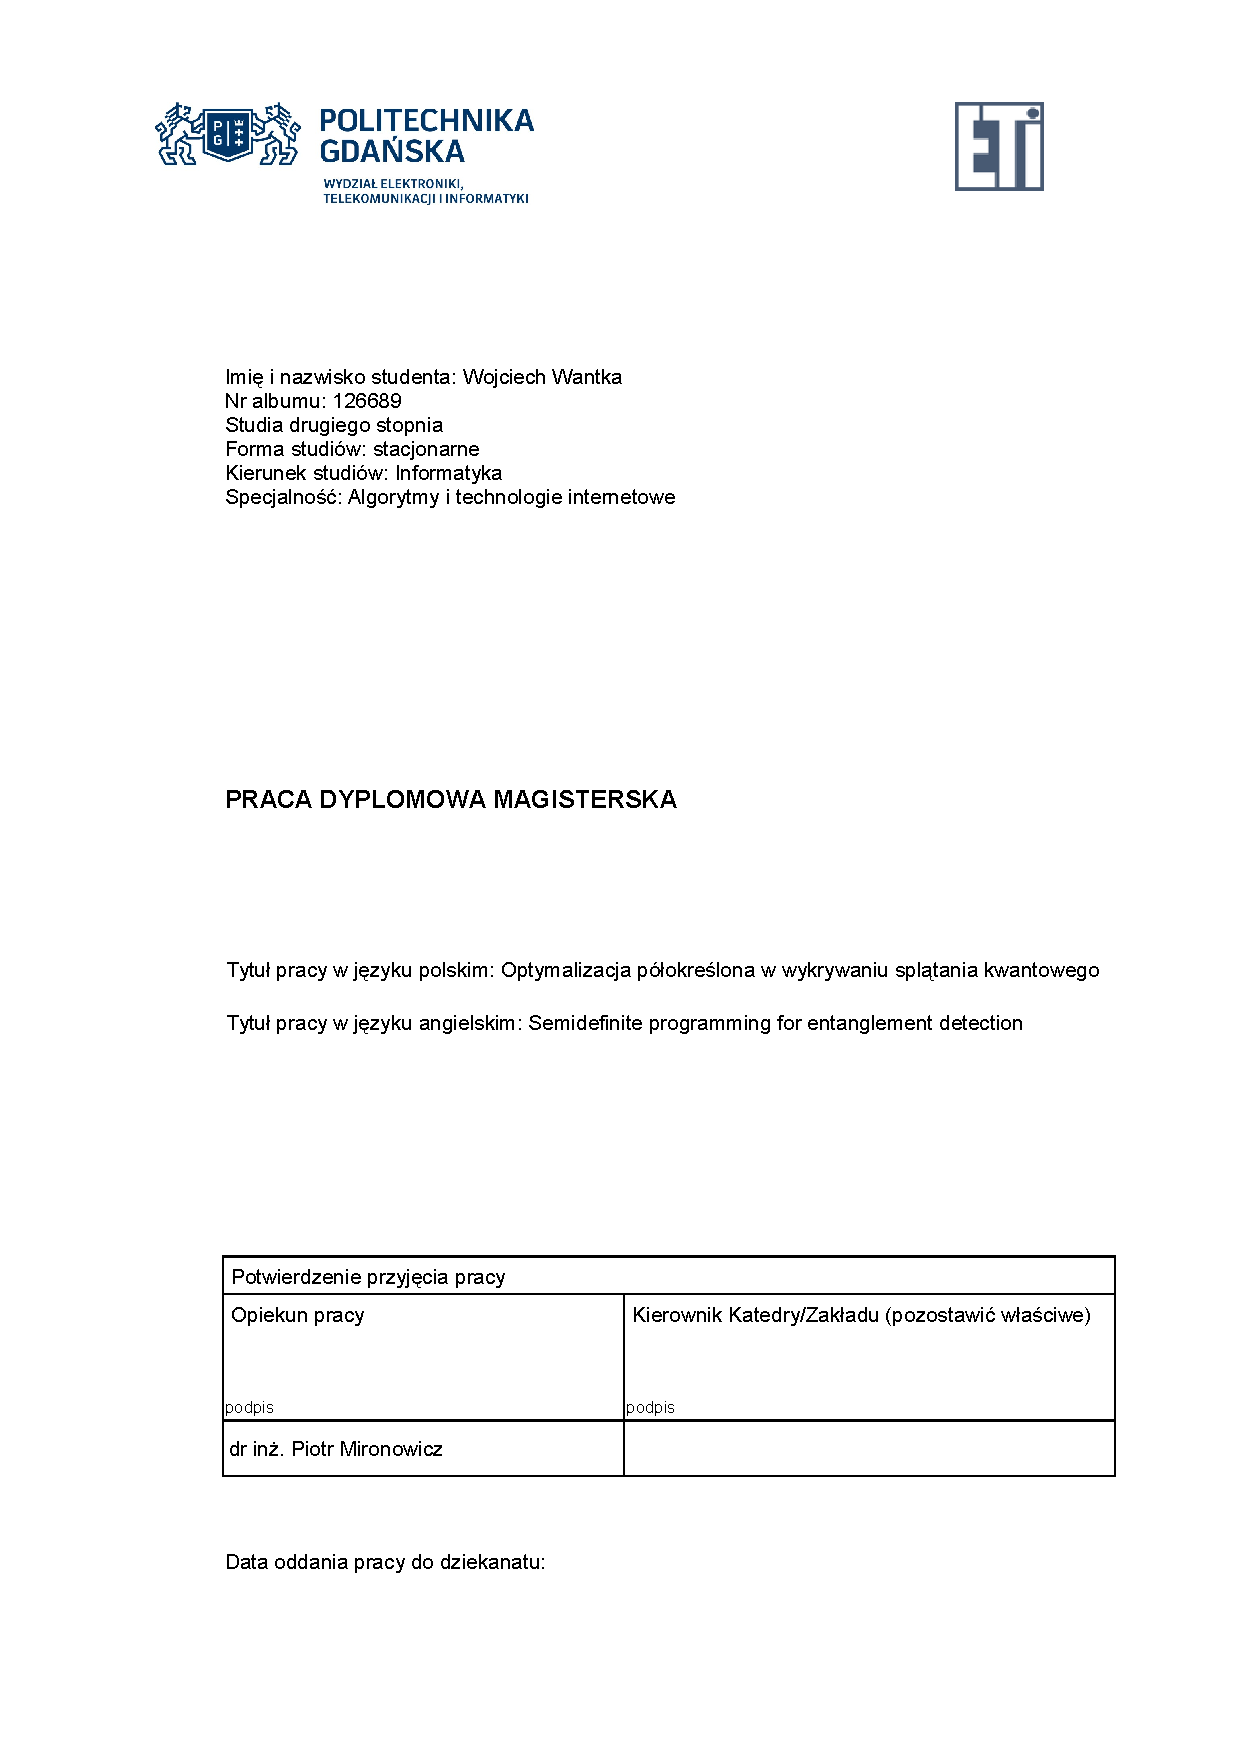
\includepdf{organizational/titlepage.pdf}

\includepdf{organizational/declaration.pdf}

\setcounter{page}{3}

\section*{Streszczenie}

W pracy przedstawiono podstawy programowania półokreślonego oraz problematykę separowalności macierzy gęstości, wraz z podaniem niezbędnej wiedzy z algebry liniowej. Praca objęła implementację potrzebnych narzędzi do formułowania warunków separowalności macierzy w oparciu o framework (np. pakiety SeDuMi i YALMIP w środowisku MATLAB/OCTAVE) oraz zilustrowanie zastosowań tych narzędzi na zaproponowanych przykładach.

Wykonane zadania:

\begin{enumerate}
    \item Przegląd literatury odnośnie programowania półokreślonego
    \item Wprowadzenie do metod informatyki kwantowej
    \item Implementacja narzędzia w postaci skryptów w języku MATLAB
    \item Sporządzenie dokumentacji skryptów oraz przykładów
\end{enumerate}

\noindent \textbf{Słowa kluczowe:} informatyka kwantowa

\noindent \textbf{Dziedzina nauki:} Nauki o komputerach i informatyka
 \newpage
\section*{Abstract}

In the thesis presented the methods of semidefinite programming and the problem of separability of density matrices, with presenting fundamental knowledge on linear algebra. The thesis includes the implementation of necessary tools formulating conditions for matrix separation based on available frameworks (e.g. SeDuMi and YALMIP packages in MATLAB/OCTAVE) and illustrated the use of these tools with proposed examples.

Tasks done:

\begin{enumerate}
    \item Overview of the literature on semidefinite programming
    \item Introduction to quantum information
    \item Implementation of tools as scripts in MATLAB
    \item Documentation of scripts and examples of their applications
\end{enumerate}

\noindent \textbf{Keywords:} quantum information

\noindent \textbf{Field of science and keywords:} Computer and information sciences
 \newpage
\renewcommand{\baselinestretch}{1.0} \normalsize % make singular leading line in table of contents
\tableofcontents
\renewcommand{\baselinestretch}{1.5} \normalsize
 \newpage
\section*{Wykaz ważniejszych oznaczeń i skrótów}
\addcontentsline{toc}{section}{Wykaz ważniejszych oznaczeń i skrótów}

$[n]$ -- dla liczby naturalnej $n$ oznacza zbiór $\{0, 1, \ldots, n - 1\}$

$V^{n}(\mathbb{C})$ -- przestrzeń liniowa wymiaru $n$ nad ciałem liczb zespolonych

$M_{n \cross m}(\mathbb{C})$ -- przestrzeń macierzy wymiaru $n \cross m$ nad ciałem liczb zespolonych

$\textbf{S} ^ {n}$ -- przestrzeń macierzy symetrycznych o wymiarze $n$ o współczynnikach rzeczywistych

$\mathcal{H}$ -- przestrzeń Hilberta

$\ket{\psi}$ -- wektor ket

$\bra{\psi}$ -- wektor bra

$\bra{\psi}\ket{\phi}$ -- iloczyn skalarny wektorów $\ket{\psi}$ i $\ket{\phi}$

$||\psi||$ -- norma wektora $\ket{\psi}$

$\ket{\psi} \otimes \ket{\phi}$ -- iloczyn tensorówy wektorów $\ket{\psi}$ i $\ket{\phi}$

$[A, B]$ -- komutator operatorów $A$ i $B$

$\textbf{Tr}[A]$ -- ślad operatora $A$
 \newpage
\section{Podstawy algebraiczne}

\subsection{Przestrzeń Hilberta}

Weźmy przestrzeń liniową wymiaru $n$ nad $\mathbb{C}$ i wyposażmy ją w iloczyn skalarny. Tak powstałą strukturę nazwiemy \textit{przestrzenią Hilberta} (ogólnie, tzn. nie skonkretyzowaną w żaden sposób przestrzeń Hilberta oznaczać będziemy $\mathcal{H}$). Element (wektor) tej przestrzeni oznaczamy $\ket{\psi}$, natomiast iloczyn skalarny pomiędzy dwoma wektorami $\ket{\psi}, \ket{\phi} \in \mathcal{H}$ oznaczymy $\bra{\psi}\ket{\phi}$ (taka konwencja określana jest mianem \textit{notacji Diraca}). Przypomnijmy jeszcze, że na przestrzeni Hilberta indukowana jest za pomocą iloczynu skalarnego \textit{norma} wektora, standardowo $||\psi|| \equiv \sqrt{\bra{\psi}\ket{\psi}}$.

\subsubsection{Baza kanoniczna}

Jako $\mathcal{B} \equiv \{\ket{i}\}_{i\in I}$ oznaczmy bazę przestrzeni $\mathcal{H}$. Zakładamy też, że $\mathcal{B}$ stanowi ortonormalny układ wektorów -- w przestrzeniach o skończonym wymiarze jesteśmy bowiem w stanie zastosować procedurę Grama-Schmidta. Dla ustalenia uwagi przyjmijmy $I \equiv \{0,1, \ldots , n - 1 \}$ -- przy takich oznaczeniach bazę $\mathcal{B}$ nazywamy bazą \textit{kanoniczną}. Przyjmuje się, że wektory bazy kanonicznej oznaczamy

$$
    \ket{i} \equiv
    \begin{pmatrix}
        0 \\
        \vdots \\
        0 \\
        1 \\
        0 \\
        \vdots \\
        0
    \end{pmatrix},
$$

gdzie nad współczynnikiem $1$ znajduje się $i$ zer.

Dowolny wektor $\ket{\psi} \in \mathcal{H}$ zapiszemy teraz jako

$$
    \ket{\psi} = \sum\limits_{i \in I} \psi_{i}\ket{i}.
$$

Założenie o skończonym wymiarze przestrzeni skutkuje wygodną reprezentacją w bazie $\mathcal{B}$ abstrakcyjnego wektora z przestrzeni Hilberta jako kolumny jego współczynników: 

$$
    \ket{\psi} \equiv
    \begin{pmatrix}
        \psi_{0} \\
        \psi_{1} \\
        \vdots \\
        \psi_{n - 1} \\
    \end{pmatrix}.
$$

\subsubsection{Współczynniki wektora w bazie ortonormalnej}
\label{coefficients}

Przypomnimy obecnie wzór na współczynniki wektora w rozwinięciu w bazie $\mathcal{B}$, która zgodnie z założeniem stanowi układ ortonormalny, tzn. 

$$
    \bra{i}\ket{j} = \delta_{ij},
$$

gdzie dwuargumentowa funkcja $\delta_{ij}$, zwana \textit{deltą Kroneckera}:

$$
    \delta_{ij} \equiv
    \begin{cases}
        1, \text{dla } i = j \\
        0, \text{dla } i \neq j
    \end{cases}
$$

Niech więc dowolnie ustalony wektor bazowy $\ket{\alpha}$ zostanie przemnożony skalarnie przez wektor $\ket{\psi}$. Pamiętając o własnościach iloczynu skalarnego (liniowość w drugim składniku) napiszemy 

$$
    \bra{\alpha}\ket{\psi} = \bra{\alpha}\left(\sum\limits_{i}\psi_{i}\ket{i}\right) = \sum\limits_{i}\psi_{i} \bra{\alpha}\ket{i} = \sum\limits_{i}\psi_{i}\delta_{\alpha i}=\psi_{\alpha}
$$

tzn.

$$
    \psi_{\alpha}=\bra{\alpha}\ket{\psi}.
$$

\subsubsection{Iloczyn skalarny -- równoważne podejście}

Iloczyn skalarny wektorów $\ket{\psi}, \ket{\phi} \in \mathcal{H}$ można wyznaczyć wprost z definicji funkcji $\bra{\psi}\ket{\phi}$, a także za pomocą sumy współczynników tych wektorów. Dla

$$
    \ket{\psi} = \sum\limits_{i\in I}\psi_{i}\ket{i}
$$

oraz

$$
    \ket{\phi} = \sum\limits_{i\in I}\phi_{i}\ket{i}
$$

mamy bowiem

$$
    \bra{\psi}\ket{\phi} = \left(\sum\limits_{i \in I}\psi_{i}\bra{i}\right)\left(\sum\limits_{j\in I}\phi_{j}\ket{j}\right) = \sum\limits_{i, j \in I}\psi_{i} ^ {*}\phi_{j}\bra{i}\ket{j}=\sum\limits_{i \in I}\psi_{i}^{*}\phi_{i}
$$

\subsubsection{Przestrzeń sprzężona}

Samo wyrażenie $\bra{\psi}\ket{\phi}$ także w konwencji Diraca traktować można dwojako -- formalnie bowiem w drugim składniku iloczynu skalarnego występują wektory postaci $\ket{\cdot}$ rozpatrywanej przestrzeni Hilberta $\mathcal{H}$, nazywane \textit{ketami}, natomiast w pierwszym -- wektory zapisywane jako $\bra{\cdot}$, nazywane \textit{bra} (oba te pojęcia pochodzą od słowa \textit{bracket}). Wektory \textit{bra} definiuje się ściśle jako elementy \textit{przestrzeni sprzężonej} do przestrzeni $\mathcal{H}$.

\begin{definition}
    Przestrzenią sprzężoną do przestrzeni Hilberta $\mathcal{H}$ nazywamy przestrzeń $\mathcal{H}^{*}$ liniowych funkcjonałów $\bra{\cdot} : \mathcal{H} \rightarrow \mathbb{C}$.
\end{definition}

\begin{remark} 
    Funkcjonały z przestrzeni sprzężonej są liniowe, ponieważ iloczyn skalarny jest liniowy w drugim argumencie.
\end{remark}

Okazuje się, że w przestrzeniach Hilberta o wymiarze skończonym występuje wzajemna jednoznaczność bra i ketów, tzn. wektor $\ket{\psi} \in \mathcal{H}$ można rozpatrywać równoważnie jako wektor $\bra{\psi} \in \mathcal{H}^{*}$ powstały z $\ket{\psi}$ na drodze przekształcenia, które w przestrzeniach o skończonym wymiarze wygląda następująco: z reprezentacji wektora jako kolumny współczynników i z formuły na iloczyn skalarny w bazie ortonormalnej mamy, że dla danego keta 

$$
    \ket{\psi} =
    \begin{pmatrix}
        \psi_{0} \\
        \psi_{1} \\
        \vdots \\
        \psi_{n - 1} \\
    \end{pmatrix}
$$
 
odpowiadający mu funkcjonał $\bra{\psi} \in \mathcal{H}^{*}$ można zapisać jako 

$$
    \bra{\psi} = \begin{pmatrix} \psi_{0}^{*} & \psi_{1}^{*} & \ldots & \psi_{n - 1}^{*} \end{pmatrix}.
$$

Wobec tego, bra powstaje z keta na skutek transpozycji i sprzężenia zespolonego. Teraz iloczyn skalarny $\bra{\psi}\ket{\phi}$ wektorów $\ket{\psi}, \ket{\phi} \in \mathcal{H}$ uzyskuje dodatkowy sens zwykłego mnożenia wiersza przez kolumnę.

\subsubsection{Podstawowe bazy}

Podamy definicje podstawowych baz pojawiających się w kwantowej informatyce.

\begin{definition}[Baza Hadamarda]
    $$
        \ket{0'} = \frac{1}{\sqrt{2}} \ket{0} + \frac{1}{\sqrt{2}} \ket{1}
    $$

    $$
        \ket{1'} = \frac{1}{\sqrt{2}} \ket{0} - \frac{1}{\sqrt{2}} \ket{1}
    $$
\end{definition}

\begin{definition}[Baza Bella]
    $$
        \ket{\Phi ^ {+}} = \frac{1}{\sqrt{2}} (\ket{00} + \ket{11}) = \frac{1}{\sqrt{2}} (\ket{0} + \ket{3})
    $$

    $$
        \ket{\Phi ^ {-}} = \frac{1}{\sqrt{2}} (\ket{00} - \ket{11}) = \frac{1}{\sqrt{2}} (\ket{0} - \ket{3})
    $$

    $$
        \ket{\Psi ^ {+}} = \frac{1}{\sqrt{2}} (\ket{01} + \ket{10}) = \frac{1}{\sqrt{2}} (\ket{1} + \ket{2})
    $$

    $$
        \ket{\Psi ^ {-}} = \frac{1}{\sqrt{2}} (\ket{01} - \ket{10}) = \frac{1}{\sqrt{2}} (\ket{1} - \ket{2})
    $$
\end{definition}

\subsection{Przestrzeń Hilberta-Schmidta}

Dla danej przestrzeni Hilberta $\mathcal{H}$ z bazą $\mathcal{B}$ wprowadzamy przestrzeń operatorów liniowych $A: \mathcal{H} \rightarrow \mathcal{H}$ z działaniem standardowego dodawania dwóch operatorów i działaniem mnożenia operatora przez liczbę zespoloną. Przestrzeń taka jest przestrzenią liniową. Wyposażamy ją w działanie dwuargumentowe postaci

$$
    \bra{A}\ket{B} \equiv \textbf{Tr}[A ^ {\dag} B].
$$

Łatwo pokazać, że tak zdefiniowana funkcja jest iloczynem skalarnym (nazywamy ją iloczynem skalarnym Hilberta--Schmidta) -- przestrzeń operatorów rozszerzyliśmy wobec tego do przestrzeni Hilberta. Nazywamy ją przestrzenią Hilberta-Schmidta sprzężoną z przestrzenią $\mathcal{H}$ i oznaczamy $\mathcal{HS}$.

\subsubsection{Elementy macierzowe, ślad, komutator}

Przedstawimy podstawowe definicje i własności operatorów.

\begin{definition}
    \label{definition:matrix-element}
    Elementem macierzowym w bazie $\mathcal{B}$ operatora liniowego $A$ nazywamy liczbę

    $$
        A_{ij} \equiv \bra{i} A \ket{j},
    $$

    gdzie $\ket{i}, \ket{j} \in \mathcal{B}$. Ponadto, elementy macierzowe postaci $A_{ii}$ nazywamy elementami diagonalnymi operatora $A$.
\end{definition}

Operator $A$ można zapisać w następujący sposób:

$$
    A = \sum\limits_{i, j \in I} A_{ij} \ket{i}\bra{j}.
$$

\begin{remark}
    Zapis postaci $\bra{\cdot}\cdot\ket{\cdot}$ stosujemy w celach mnemotechnicznych -- obowiązuje tutaj ogólna konwencja notacyjna:

    \begin{itemize}
        \item $\ket{A \psi} \equiv A \ket{\psi}$
        \item $\bra{A \psi} \equiv \bra{\psi} A ^ {\dag}$
    \end{itemize}
\end{remark}

\begin{definition}[Ślad operatora]
    Śladem operatora liniowego $A$ nazywamy sumę jego elementów diagonalnych:

    $$
        \textbf{Tr}[A] \equiv \sum\limits_{i \in I} A_{ii}.
    $$
\end{definition}

\begin{theorem}[Ślad operatora jest cykliczny]
    Zachodzi

    $$
        \textbf{Tr}[AB] = \textbf{Tr}[BA]
    $$
\end{theorem}

Wprowadzimy teraz pojęcie \textit{komutatora} operatorów liniowych.

\begin{definition}[Komutator]
    Dla operatorów liniowych $A$ oraz $B$ działających na przestrzeni Hilberta $\mathcal{H}$ ich komutator definiujemy jako operator liniowy

    $$
        [A, B] \equiv A \circ B - B \circ A,
    $$

    gdzie działanie $\circ$ oznacza złożenie operatorów (w przypadku skończenie wymiarowym i reprezentacji macierzowej operatora jest to mnożenie macierzy). Ponadto, jeżeli $[A, B] = \hat{0}$ (gdzie $\hat{0}$ jest operatorem zerowym) to mówimy, że operatory $A$ i $B$ komutują.

\end{definition}

\subsubsection{Operatory hermitowskie}

Wprowadzimy pojęcie operatora hermitowskiego i podamy jego podstawowe własności.

\begin{definition}[Sprzężenie hermitowskie]
    Niech $\ket{\psi}, \ket{\phi} \in \mathcal{H}$, natomiast $A$ niech jest operatorem liniowym z $\mathcal{H}$ do $\mathcal{H}$. Operatorem sprzężonym hermitowsko do $A$ nazywamy operator 

    $$
        A ^ {\dag} \equiv (A ^ {*}) ^ T = (A ^ {T}) ^ {*}.
    $$
\end{definition}

\begin{definition}[Operator hermitowski]
    Operator liniowy $A$ nazywamy hermitowskim (samosprzężonym), gdy

    $$
        A = A ^ {\dag}
    $$
\end{definition}

\begin{theorem}
    Wartości własne operatora hermitowskiego są rzeczywiste.
\end{theorem}

\subsubsection{Operatory dodatnio określone}

Wprowadzimy pojęcie i podamy podstawowe własności operatorów dodatnio określonych.

\begin{definition}[Operator dodatnio określony]
    \label{definition:semidefinite}
    Operator liniowy $A$ nazywamy dodatnio określonym, gdy

    $$
        \forall_{\ket{\psi} \in \mathcal{H}} \bra{\psi} A \ket{\psi} \geq 0.
    $$

    Piszemy wtedy $A \geq 0$.
\end{definition}

\begin{theorem}
    \label{theorem:positive}
    Operator dodatnio określony jest hermitowski.
\end{theorem}

\begin{theorem}
    \label{theorem:positivevalues}
    Wartości własne operatora dodatnio określonego są nieujemnymi liczbami rzeczywistymi.
\end{theorem}

\begin{theorem}
    \label{theorem:adaga}
    Jeżeli $A$ jest operatorem liniowym, to operator $A ^ {\dag} A$ jest dodatnio określony.
\end{theorem}

\begin{proof}
    Niech $\ket{\psi} \in \mathcal{H}$ będzie dowolnym wektorem. Wtedy

    $$
        \bra{\psi} A ^ {\dag} A \ket{\psi} = \bra{A \psi}\ket{A \psi}=\left\|A \ket{\psi}\right\|^2 \geq 0,
    $$

    więc $A ^ {\dag} A$ jest operatorem dodatnio określonym.
\end{proof}

\begin{theorem}
    Jeżeli $A$, $B$ są operatorami na $\mathcal{H}$ dodatnio określonymi, to ich suma $A + B$ jest operatorem dodatnio określonym.
\end{theorem}

\begin{proof}
    Niech $\ket{\psi} \in \mathcal{H}$. Wtedy

    $$
        \bra{\psi} (A + B) \ket{\psi}=\bra{\psi} A \ket{\psi} + \bra{\psi} B \ket{\psi} \geq 0.
    $$
\end{proof}

Jako definicję operatora dodatnio określonego równoważną definicji \ref{definition:semidefinite} można przyjąc poniższą definicję \textit{operatora dodatniego} (nazwa została przyjęta jedynie po to, aby odróżnić od siebie dokładne treści obu definicji):

\begin{definition}[Operator dodatni]
    Operator liniowy $A$ nazywamy dodatnim, gdy jest hermitowski i ma nieujemne spektrum.
\end{definition}

Okazuje się bowiem, że z twierdzeń \ref{theorem:positive} oraz \ref{theorem:positivevalues}  wynika

\begin{corollary}
    \label{corollary:iff}
    Operator liniowy $A$ jest dodatnio określony $\Longleftrightarrow$ jest dodatni.
\end{corollary}

\subsection{Iloczyn tensorowy}

\subsubsection{Definicja ogólna}

W niniejszym paragrafie postaramy się przedstawić w możliwie najogólniejszy sposób definicję iloczynu tensorowego, podając następnie praktyczną jego realizację w przestrzeniach o wymiarze skończonym.

Weźmy dwie przestrzenie Hilberta $\mathcal{H}_{A}$ i $\mathcal{H}_{B}$. Dla wektorów $\ket{A} \in \mathcal{H}_{A}$ oraz $\ket{B} \in \mathcal{H}_{B}$ wektor będący ich \textit{iloczynem tensorowym} (oznaczany $\ket{A} \otimes \ket{B}$) formalnie jest elementem przestrzeni będącej \textit{iloczynem tensorowym przestrzeni} $\mathcal{H}_{A}$ i $\mathcal{H}_{B}$. Najpierw wprowadzimy więc pojęcie iloczynu tensorowego przestrzeni, a następnie -- definicję działania mnożenia tensorowego wektorów.

\begin{definition}[Iloczyn tensorowy przestrzeni]
    Iloczynem tensorowym przestrzeni Hilberta $\mathcal{H}_A$ (z ortonormalną bazą $\ket{i^{A}}$) i $\mathcal{H}_B$ (z ortonormalną bazą $\ket{j^{B}}$) nazywamy przestrzeń

    $$
        \mathcal{H}_{AB} \equiv \mathcal{H}_A \otimes \mathcal{H}_B,
    $$

    której elementy stanowią wszystkie wektory postaci

    \begin{equation}
        \label{equation:product}
        \ket{C} \equiv \ket{A} \otimes \ket{B}, \textrm{dla } \ket{A} \in \mathcal{H}_A, \ket{B} \in \mathcal{H}_B.
    \end{equation}

    Dodatkowo, wektory tej przestrzeni stanowią z definicji wszystkie kombinacje liniowe układu wektorów $\left|i^{A}\right\rangle\otimes\left|j^{B}\right\rangle$, tzn. zbiór wektorów postaci

    \begin{equation}
        \label{equation:entangled}
        \ket{C} = \sum\limits_{ij} c_{ij} \ket{i ^ {A}} \otimes \ket{j ^ {B}}.
    \end{equation}
\end{definition}

\begin{definition}[Iloczyn tensorowy wektorów]
    Dla danych przestrzeni Hilberta $\mathcal{H}_A$ oraz $\mathcal{H}_B$ działanie mnożenia tensorowego wektorów z $\mathcal{H}_A$ z wektorami z $\mathcal{H}_B$ definiuje się jako funkcję $\otimes: \mathcal{H}_A \times \mathcal{H}_B \rightarrow \mathcal{H}_{AB}$, mającą własność liniowości w obu swoich składnikach, tzn.

    \begin{enumerate}
        \item \textbf{Jednorodność w obu składnikach.}
            Dla każdego skalara $z \in \mathbb{C}$ i dla każdych wektorów $A \in \mathcal{H}_A$ oraz $B \in \mathcal{H}_B$

            $$
                z (\ket{A} \otimes \ket{B}) = (z \ket{A}) \otimes \ket{B} = \ket{A} \otimes (z \ket{B})
            $$
        \item \textbf{Addytywność w pierwszym składniku.}
            Dla każdych wektorów $\ket{A_1}, \ket{A_2} \in \mathcal {H}_A$ oraz $\ket{B} \in \mathcal{H}_B$

            $$
                (\ket{A_1} + \ket{A_2}) \otimes \ket{B} = \ket{A_1} \otimes \ket{B} + \ket{A_2} \otimes \ket{B}
            $$
        \item \textbf{Addytywność w drugim składniku.}
            Dla każdych wektorów $\ket{A} \in \mathcal{H}_A$ oraz $\ket{B_1}, \ket{B_2} \in \mathcal{H}_B$

            $$
                \ket{A} \otimes (\ket{B_1} + \ket{B_2}) = \ket{A} \otimes \ket{B_1} + \ket{A} \otimes \ket{B_2}
            $$
    \end{enumerate}
\end{definition}

\begin{remark}[Oznaczenia]
    Dla $\ket{A} \in \mathcal{H}_{A}$ i $\ket{B} \in \mathcal{H}_{B}$ oznaczać będziemy 

    $$
        \ket{A} \otimes \ket{B} \equiv \ket{A} \ket{B}.
    $$

    Czasem piszemy nawet $\ket{A} \otimes \ket{B} \equiv \ket{A B}$.
\end{remark}

\begin{remark}
    \label{remark:classes}
    Z liniowości iloczynu tensorowego wynika, że każdy wektor z $\mathcal{H}_{AB}$ postaci (\ref{equation:product}) można zapisać w postaci (\ref{equation:entangled}). Dla

    $$
        \ket{A} = \sum\limits_{i} c_i ^ {(A)} \ket{i^{(A)}}
    $$

    oraz

    $$
        \ket{B} = \sum\limits_{j} c_j ^ {(B)} \ket{j^{(B)}}
    $$

    mamy bowiem

    $$
        \ket{A} \ket{B} = \left(\sum\limits_{i} c_i ^ {(A)} \ket{i^{(A)}}\right) \left(\sum\limits_{j} c_j ^ {(B)} \ket{j^{(B)}}\right)
    $$

    $$
        = \sum\limits_{ij} c_{i} ^ {(A)} c_{j} ^ {(B)} \ket{i ^ {(A)}} \ket{j ^ {(B)}} = \sum\limits_{ij} c_{ij} \ket{i ^ {(A)}} \ket{j ^ {(B)}},
    $$

    jeżeli tylko $c_{ij} \equiv c_{i} ^ {(A)} c_{j} ^ {(B)}$.

    Implikacja odwrotna jednak nie zachodzi: nie każdy wektor dany w postaci (\ref{equation:entangled}) da się zapisać w postaci (\ref{equation:product}) (podamy później przykład takiego wektora). Ta własność zdefiniowanej przez nas struktury iloczynu tensorowego będzie miała wielkie znaczenie przy wprowadzaniu pojęcia \textit{splątania}.
\end{remark}

\begin{remark}
    \label{remark:product-vector}
    O tych wektorach przestrzeni $\mathcal{H}_{AB}$, które można zapisać w postaci (\ref{equation:product}) mówimy, że są wektorami produktowymi.
\end{remark}

\subsubsection{Iloczyn tensorowy w przestrzeniach o skończonym wymiarze}

Podamy teraz definicję iloczynu tensorowego w przestrzeniach Hilberta o wymiarze skończonym określonych nad $\mathbb{C}$.

Wprowadzimy najpierw pewne działanie wykonywane na macierzach -- rozważane ogólnie nie ma ono nic wspólnego z teorią kwantów.

\begin{definition}[Iloczyn Kroneckera macierzy]
    Dla macierzy

    $$
        A \in M_{p \times q}(\mathbb{C})
    $$

    i

    $$
        B \in M_{r\times s}(\mathbb{C})
    $$

    ich iloczyn Kroneckera zdefiniowany jest jako macierz

    $$
        C \in M_{pr\times qs}(\mathbb{C})
    $$

    dana wzorem

    \begin{equation}
        \label{equation:kronecker-product}
        C \equiv A \otimes B =
        \begin{pmatrix}
            A_{00} B & A_{01} B & \ldots & A_{0, q - 1} B \\
            A_{10} B & A_{11} B & \ldots & A_{1, q - 1} B \\
            \vdots & \vdots & \vdots & \vdots \\
            A_{p - 1, 0} B & A_{p - 1, 1} B & \ldots & A_{p - 1, q - 1} B
        \end{pmatrix}.
    \end{equation}
\end{definition}

\begin{example}[Iloczyn Kroneckera]
    Dla danych macierzy

    $$
        A =
        \begin{pmatrix}
            a & b \\
            c & d
        \end{pmatrix}
    $$

    $$
        B =
        \begin{pmatrix}
            e & f & g \\
            h & i & j
        \end{pmatrix}
    $$

    ich iloczyn Kroneckera przyjmuje wartość

    $$
        C =
        \begin{pmatrix}
            a B & b B \\
            c B & d B
        \end{pmatrix}
        =
        \begin{pmatrix}
            a e & a f & a g & b e & b f & b g \\
            a h & a i & a j & b h & b i & b j \\
            c e & c f & c g & d e & d f & d g \\
            c h & c i & c j & d h & d i & d j
        \end{pmatrix}
    $$
\end{example}

Podamy podstawowe własności iloczynu Kroneckera.

\begin{theorem}
    Jeżeli $A$, $B$, $C$, $D$ są macierzami takimi, że wyrażenia $A C$ i $B D$ mają sens jako mnożenie algebraiczne macierzy, to

    \begin{equation}
        (A \otimes B) (C \otimes D) = (A C) \otimes (B D),
    \end{equation}

    gdzie $\otimes$ jest iloczynem Kroneckera macierzy.
\end{theorem}

Można też udowodnić twierdzenie ogólniejsze:

\begin{theorem}
    \label{theorem:generic}
    Niech $\ket{a_{1}}, \ket{a_{2}} \in \mathcal{H}_{A}$, $\ket{b_{1}}, \ket{b_{2}} \in \mathcal{H}_{B}$. Wówczas

    \begin{equation}
        (\ket{a_{1}} \ket{b_{1}}) (\bra{a_{2}} \bra{b_{2}}) = \ket{a_{1}} \bra{a_{2}} \otimes \ket{b_{1}} \bra{b_{2}}.
    \end{equation}
\end{theorem}

Ponadto mamy

\begin{theorem}
    Jeżeli $A$, $B$ są macierzami, to

    \begin{equation}
        (A \otimes B) ^ {\dag} = A ^ \dag \otimes B ^ \dag.
    \end{equation}
\end{theorem}

\begin{corollary}
    Iloczyn Kroneckera zachowuje hermitowskość, tzn. jeżeli macierze $A$ i $B$ są hermitowskie, to macierz $A \otimes B$ również.
\end{corollary}

Można też pokazać, że w odniesieniu do operatora \textbf{Tr} mamy następujące

\begin{theorem}
    Jeżeli $A$ i $B$ są dowolnymi macierzami kwadratowymi, to

    \begin{equation}
        \textbf{Tr}[A \otimes B] = \textbf{Tr}[A] \cdot \textbf{Tr}[B].
    \end{equation}
\end{theorem}

Należy podkreślić, że działanie (\ref{equation:kronecker-product}) \textit{spełnia własności iloczynu tensorowego}. Pokażemy później, że w kwantowej teorii informacji interesującymi nas przestrzeniami Hilberta są zwykłe $n$-wymiarowe przestrzenie kolumn liczb zespolonych $V ^ n (\mathbb{C})$ i sprzężone z nimi przestrzenie Hilberta--Schmidta, tzn. przestrzenie macierzy kwadratowych wymiaru $n$: $M_{n\times n}(\mathbb{C})$. Naturalnym rozwiązaniem jest przyjęcie w tych przestrzeniach iloczynu tensorowego według reguły (\ref{equation:kronecker-product}). Wobec tego, w kwantowej teorii informacji iloczyn tensorowy oznacza po prostu iloczyn Kroneckera.

Uogólnimy obecnie rozważania podane w definicji \ref{definition:matrix-element}.

Niech dane są skończenie wymiarowe przestrzenie Hilberta $\mathcal{H}_{A}$ oraz $\mathcal{H}_{B}$ z bazami odpowiednio

$$
    \{\ket{a_{i}}\}_{i \in [n_{A}]}
$$

oraz

$$
    \{\ket{b_{j}}\}_{j \in [n_{B}]}.
$$

Niech dany jest też operator liniowy $A$ działający na przestrzeni $\mathcal{H}_{A} \otimes \mathcal{H}_{B}$. Dla

$$
    i, k \in [n_{A}],
$$

$$
    j,l \in [n_{B}]
$$

elementem macierzowym tego operatora w bazie $\{\ket{a_{i}} \ket{b_{j}}\}_{i \in [n_{A}], j \in [n_{B}]}$ przestrzeni złożonej nazywamy liczbę

$$
    A_{\stackrel{ij}{kl}} \equiv \bra{a_{i}} \bra{b_{j}} A \ket{a_{k}} \ket{b_{l}}.
$$

Operator $A$ zapiszemy wtedy w rozważanej bazie jako

$$
    A = \sum\limits_{i, k \in [n_{A}]; j, l \in [n_{B}]} A_{\stackrel{ij}{kl}} (\ket{a_{i}} \ket{b_{j}}) (\bra{a_{k}} \bra{b_{l}})
$$

\begin{equation}
    \label{equation:elements}
    \stackrel{Tw. \ref{theorem:generic}}{=} \sum\limits_{i, k \in [n_{A}]; j, l \in [n_{B}]} A_{\stackrel{ij}{kl}} \ket{a_{i}} \bra{a_{k}} \otimes \ket{b_{j}} \bra{b_{l}}.
\end{equation}

\subsection{Twierdzenie spektralne}

\subsubsection{Projektory}

\begin{definition}
    Niech $\mathcal{H}_{A}$, $\mathcal{H}_{B}$ będą skończenie wymiarowymi przestrzeniami Hilberta. Dla $\ket{A} \in \mathcal{H}_A$ i $\ket{B} \in \mathcal{H}_B$ wyrażenie $\ket{A} \bra{B}$ wyznaczone według reguły (\ref{equation:kronecker-product}) i będące wektorem z przestrzeni $\mathcal{H}_A \otimes \mathcal{H}_{B} ^ {*}$, gdzie $\mathcal{H}_{B} ^ {*}$ jest przestrzenią sprzężoną do przestrzeni $\mathcal{H}_B$, nazywamy iloczynem zewnętrznym wektorów $\ket{A}$ i $\ket{B}$.
\end{definition}

Niech dana jest przestrzeń Hilberta $\mathcal{H}$ wymiaru $n$ z bazą ortonormalną $\{\ket{i}\}_{i = 0} ^ {n - 1}$. Wtedy (zob. \ref{coefficients}) dowolny wektor $\ket{\psi} \in \mathcal{H}$ można zapisać jako

$$
    \ket{\psi} = \sum\limits_{i = 0} ^ {n - 1} \ket{i} \underbrace{\bra{i}\ket{\psi}}_{\psi_{i}}.
$$

Każdemu wektorowi $\ket{i}$ z bazy przypiszmy teraz operator liniowy $\ket{i} \bra{i} : \mathcal{H} \rightarrow \mathcal{H}$, którego działanie zdefiniujemy następująco:

$$
    (\ket{i} \bra{i}) \ket{\psi} \equiv \ket{i} \bra{i}\ket{\psi}.
$$

Wtedy

$$
    \ket{\psi} = \left(\sum_{i = 0} ^ {n - 1} \ket{i} \bra{i} \right) \ket{\psi},
$$

tzn.

\begin{equation}
    \label{equation:identity}
    \sum\limits_{i = 0} ^ {n - 1} \ket{i} \bra{i} = I.
\end{equation}

Oznaczmy

$$
    \Pi_{i} \equiv \ket{i} \bra{i}, i = 0, 1, \ldots, n - 1.
$$

\begin{definition}
    Niech dana jest przestrzeń liniowa i jej podprzestrzeń $V$. Niech bazą podprzestrzeni $V$ jest $\mathcal{B}_{V}$. Projektorem rzutującym na podprzestrzeń $V$ nazywamy operator

    $$
        \Pi_V \equiv \sum\limits_{\ket{i} \in \mathcal{B}_V} \ket{i} \bra{i}.
    $$

    Ponadto, jeżeli baza $\mathcal{B}_V$ jest układem ortonormalnym, to projektor $\Pi_V$ nazywamy ortonormalnym.
\end{definition}

Własność (\ref{equation:identity}) układu ortonormalnych projektorów $\{\ket{i} \bra{i}\}_{i = 0} ^ {n - 1}$ nazywamy \textit{rozkładem identyczności}. Ponadto, złożenie dwóch projektorów z tego układu spełnia

$$
    \Pi_{i} \Pi_{j} = \delta_{ij} \Pi_{i}.
$$

Mamy bowiem dla dowolnego wektora $\ket{\psi} \in \mathcal{H}$

$$
    \Pi_{i} \Pi_{j} \ket{\psi} = \Pi_{i} \ket{j} \bra{j}\ket{\psi} = \ket{i} \bra{i}\ket{j} \bra{j}\ket{\psi} = \delta_{ij} \Pi_{i} \ket{\psi}.
$$

Latwo też pokazać, że konstrukcja skończenie wymiarowych projektorów ortonormalnych za pomocą iloczynu Kroneckera implikuje ich hermitowskość.

\begin{fact}
    Projektory ortonormalne są operatorami dodatnio określonymi.
\end{fact}

\begin{proof}
    Jeżeli $\Pi$ jest projektorem ortonormalnym, to

    $$
        \Pi ^ {\dag} \Pi = \Pi ^ 2 =\Pi.
    $$

    Z drugiej strony, z twierdzenia \ref{theorem:adaga} wynika, że operator $\Pi ^ {\dag} \Pi$ jest dodatnio określony.
\end{proof}

\subsubsection{Rozkład spektralny}

Przedstawimy tutaj ideę \textit{rozkładu spektralnego} operatora. Samo pojęcie zdefiniujemy rozważając przypadek, gdy działa on w pewnej przestrzeni Hilberta $\mathcal{H}$. Konstrukcję uogólnimy następnie do przestrzeni $\mathcal{H}_{AB} \equiv \mathcal{H}_A \otimes \mathcal{H}_B$.

\paragraph{Przestrzeń $\mathcal{H}$}

Rozważmy operator liniowy $A$ działający w przestrzeni Hilberta $\mathcal{H}$.

\begin{definition}
    Mówimy, że operator liniowy $A$ \textit{ma rozkład spektralny}, gdy da się go przedstawić w postaci

    $$
        A = \sum\limits_{\lambda \in \sigma(A)} \lambda \Pi_{\lambda},
    $$

    gdzie $\sigma(A)$ jest zbiorem różnych wartości własnych operatora $A$, natomiast $\Pi_{\lambda}$ jest projektorem ortonormalnym rzutującym na podprzestrzeń własną odpowiadającą wartości własnej $\lambda$.
\end{definition}

\begin{definition}[Operator normalny]
    Operator liniowy $A$ nazywamy normalnym gdy

    $$
        A ^ {\dag} A = A A ^ {\dag}
    $$
\end{definition}

\begin{theorem}[Twierdzenie Spektralne]
    \label{theorem:spectral}
    Operator liniowy ma rozkład spektralny $\Leftrightarrow$ jest normalny.
\end{theorem}

Ponieważ operator hermitowski jest normalny:

$$
    A = A ^ {\dag} \Longrightarrow A ^ {\dag} A = A A ^ {\dag} = A ^ 2,
$$

to z twierdzenia \ref{theorem:spectral} mamy

\begin{corollary}
    \label{corollary:hermitian}
    Operator hermitowski ma rozkład spektralny.
\end{corollary}

Zapiszmy jeszcze prosty fakt.

\begin{fact}
    Jeżeli operatory liniowe $A$ oraz $B$ działające na przestrzeni Hilberta $\mathcal{H}$ wymiaru $n$ posiadają rozkład spektralny we wspólnej bazie ortonormalnych projektorów $\{\Pi_{i}\}_{i = 0} ^ {n - 1}$ postaci

    $$
        A = \sum\limits_{i = 0} ^ {n - 1} a_{i} \Pi_{i},
    $$

    $$
        B = \sum\limits_{i = 0} ^ {n - 1} b_{i} \Pi_{i},
    $$

    to operatory $A$ i $B$ komutują.
\end{fact}

\begin{proof}
    Zachodzi

    $$
        A B = \left(\sum\limits_{i = 0} ^ {n - 1} a_{i} \Pi_{i}\right) \left(\sum\limits_{j = 0} ^ {n - 1} b_{j} \Pi_{j}\right) = \sum\limits_{i, j = 0} ^ {n - 1} a_{i} b_{j} \Pi_{i} \Pi_{j} = \sum\limits_{i = 0} ^ {n - 1} a_{i} b_{i} \Pi_{i}.
    $$

    Podobnie

    $$
        B A = \sum\limits_{i = 0} ^ {n - 1} b_{i} a_{i} \Pi_{i}.
    $$

    Wobec tego $A B = B A$.
\end{proof}

\paragraph{Przestrzeń $\mathcal{H}_{AB}$}

Rozważmy teraz przestrzenie Hilberta $\mathcal{H}_{A}$ oraz $\mathcal{H}_{B}$, odpowiednio wymiaru $n_{A}$ i $n_{B}$ i z bazami ortonormalnych projektorów

$$
    \left\{\Pi_{i} ^ {(A)}\right\}_{i = 0} ^ {n_{A} - 1},
$$

$$
    \left\{\Pi_{j} ^ {(B)}\right\}_{j = 0} ^ {n_{B} - 1}.
$$

Uogólnienia dokonamy dla operatorów produktowych działających w $\mathcal{H}_{AB}$, tzn. dla takich operatorów $E ^ {(AB)}$, które w przestrzeni Hilberta--Schmidta $\mathcal{HS}_{AB} \equiv \mathcal{HS}_A \otimes \mathcal{HS}_B$ sprzężonej z przestrzenią Hilberta $\mathcal{H}_{AB}$, są wektorami produktowymi (\ref{equation:product}), tzn.

$$
    E ^ {(AB)} = E ^ {(A)} \otimes E ^ {(A)},
$$

gdzie pewne operatory $E ^ {(A)}$, $E ^ {(B)}$ działające na przestrzeni $\mathcal{H}_A$ oraz $\mathcal{H}_B$ same mają rozkłady spektralne

$$
    E ^ {(A)} = \sum\limits_{i} \lambda_{i} ^ {(A)} \Pi_{i} ^ {(A)},
$$

$$
    E ^ {(B)} = \sum\limits_{j} \lambda_{j} ^ {(B)} \Pi_{j} ^ {(B)}.
$$

Wtedy

$$
    E ^ {(AB)} = \left(\sum\limits_{i} \lambda_{i} ^ {(A)} \Pi_{i} ^ {(A)}\right) \otimes \left(\sum\limits_{j} \lambda_{j} ^ {(B)} \Pi_{j} ^ {(B)}\right)
$$

$$
    = \sum\limits_{ij} \lambda_{i} ^ {(A)} \lambda_{j} ^ {(B)} \Pi_{i} ^ {(A)} \otimes \Pi_{j} ^ {(B)}.
$$

Definiując $\lambda_{ij} ^ {(AB)} \equiv \lambda_{i} ^ {(A)} \lambda_{j} ^ {(B)}$, $\Pi_{ij} ^ {(AB)} \equiv \Pi_{i} ^ {(A)} \otimes \Pi_{j} ^ {(B)}$, otrzymujemy rozkład spektralny operatora $E ^ {(AB)}$ na projektory działające w przestrzeni $\mathcal{H}_{AB}$ postaci

$$
    E ^ {(AB)} = \sum\limits_{ij} \lambda_{ij} ^ {(AB)} \Pi_{ij} ^ {(AB)},
$$

gdzie bazą ortonormalnych projektorów jest zbiór

$$
    \left\{\Pi_{ij} ^ {(AB)}\right\}_{i \in [n_{A}], j \in [n_{B}]}.
$$

\begin{remark}
    Zauważmy jednak, że niekoniecznie wszystkie tak określone wartości własne są różne.
\end{remark}

\subsection{Operatory binarne i operatory von Neumanna}

Opiszemy tutaj pewną klasę operatorów hermitowskich.

\subsubsection{Operatory binarne}

\begin{definition}[Operator binarny]
    Operator liniowy $A$ nazywamy binarnym, gdy $A$ jest hermitowski i $A ^ 2 = I$.
\end{definition}

\begin{fact}
    Jeżeli $A$ jest operatorem hermitowskim, to

    $$
        A ^ {2} = I \Longleftrightarrow \sigma(A) \subseteq \left\{+1,-1\right\}.
    $$
\end{fact}

\subsubsection{Macierze Pauliego}

\begin{definition}[Macierze Pauliego]
    Macierzami Pauliego nazywamy następujące macierze:

    $$
        \sigma_{x} =
        \begin{pmatrix}
            0 & 1 \\
            1 & 0
        \end{pmatrix}
    $$

    $$
        \sigma_{y} =
        \begin{pmatrix}
            0 & -i \\
            i & 0
        \end{pmatrix}
    $$

    $$
        \sigma_{z} =
        \begin{pmatrix}
            1 & 0 \\
            0 & -1
        \end{pmatrix}
    $$
\end{definition}

\subsubsection{Operatory von Neumanna}

\begin{definition}[Operator von Neumanna]
    Jeżeli $\hat{v} \in \mathbb{R} ^ 3$ jest wektorem jednostkowym, to operatorem von Neumanna (operatorem pomiaru spinu wzdłuż osi $\hat{v}$) nazywamy operator działający na przestrzeni $V ^ {2} (\mathbb{C})$ dany wzorem

    $$
        \hat{v} \cdot \vec{\sigma} \equiv \sum\limits_{i = 1} ^ {3} v_{i} \sigma_{i} =
        \begin{pmatrix}
            v_3 & v_{1} - i v_{2} \\
            v_{1} + i v_{2} & -v_3
        \end{pmatrix}.
    $$
\end{definition}

Przytoczymy poniżej kilka podstawowych własności operatorów von Neumana.

\begin{theorem}
    Jeżeli $\hat{a} \cdot \vec{\sigma}, \hat{b} \cdot \vec{\sigma}$ są operatorami von Neumanna, to

    $$
        (\hat{a} \cdot \vec{\sigma}) (\hat{b} \cdot \vec{\sigma}) = \left(\hat{a} \cdot \hat{b} \right) I + i \left(\hat{a} \times \hat{b}\right) \cdot \vec{\sigma}.
    $$
\end{theorem}

\begin{fact}
    Operator von Neumanna $\hat{v} \cdot \vec{\sigma}$ jest operatorem hermitowskim. Ponadto łatwo sprawdzić, że $\left(\hat{v} \cdot \vec{\sigma}\right) ^ 2 = I$. Wobec tego, $\hat{v} \cdot \vec{\sigma}$ jest operatorem binarnym.
\end{fact}

\begin{fact}
    Spektrum operatora von Neumanna $\hat{v} \cdot \vec{\sigma}$ to zbiór $\{+1, -1\}$. Ponadto

    $$
    \hat{v} \cdot \vec{\sigma} = \Pi_{+} - \Pi_{-},
    $$

    gdzie $\Pi_{\pm} = \frac{1}{2} (I \pm \hat{v} \cdot \vec{\sigma})$ jest projektorem rzutującym na odpowiednią podprzestrzeń własną.
\end{fact}
 \newpage
\subsection{Stany kwantowe}

W ujęciu ogólnym stan układu kwantowego dany jest \textit{funkcją falową}, tzn. funkcją zespoloną zależną od parametru czasu i biorącą również wartości z \textit{przestrzeni konfiguracyjnej} badanego układu (ma ona spełniać odpowiednie równanie różniczkowe -- w przypadku nierelatywistycznej mechaniki kwantowej jest to równanie Schr\"{o}dingera). Nie będziemy się tym ogólnym podejściem zajmować (jednak dla wygody także w skończonym wymiarze używać będziemy pojęcia ``funkcja falowa'' w odniesieniu do obiektu opisującego stan układu). W przypadku skończenie wymiarowym odpowiednikiem funkcji falowej jest wektor z przestrzeni $V ^ n(\mathbb{C})$ lub macierz (operator liniowy) z przestrzeni $M_{n \times n}(\mathbb{C})$. Oba przypadki rozważamy poniżej. Przyjmijmy też pewną umowę:

\begin{convention}
    \label{convention:space}
    W dalszych rozważaniach mówiąc ``przestrzeń Hilberta'' mamy na myśli przestrzeń

    \begin{equation}
        \label{equation:states}
        \mathcal{H} \equiv V^n(\mathbb{C}).
    \end{equation}

    Wtedy sprzężona z nią przestrzeń Hilberta--Schmidta

    \begin{equation}
        \label{equation:operators}
        \mathcal{HS} \equiv M_{n \times n}(\mathbb{C}).
    \end{equation}
\end{convention}

Opis przeprowadzimy dokonując podziału na układy kwantowe \textit{pojedyncze} i \textit{złożone} -- podamy matematyczną strukturę tych ostatnich. Uprzedzając jednak fakty (wynikające z tej struktury) powiedzmy najpierw, że to, czy dany obiekt matematyczny mający opisać pewien rzeczywisty układ kwantowy potraktujemy jako pojedynczy bądź złożony (w sensie poniższych definicji) można niekiedy przyjąć jako sprawę umowy (i wygody w obliczeniach). Bywa jednak też tak, że rozróżnienia dokonują same prawa fizyki i nie ma możliwości nagiąć do nich opisywanego przez nas formalizmu.

\subsubsection{Układy pojedyncze}

\paragraph{Stany czyste układów pojedynczych}

\begin{definition}[Stany czyste]
    \strut
    \begin{enumerate}
        \item Stanem czystym pojedynczego układu kwantowego nazywamy unormowany wektor

            $$
                \ket{\psi} = \sum\limits_{i} \psi_{i} \ket{i}
            $$
            z przestrzeni $\mathcal{H}$ z bazą ortonormalną

            $$
                \mathcal{B} = \{\ket{i}\}_{i \in I}, I = \{0, 1, \ldots, n - 1\},
            $$
            której elementy nazywamy \textit{stanami bazowymi}

        \item Ponadto, prawdopodobieństwo tego, że stan $\ket{\psi}$ występuje w stanie $\ket{i}$ definiuje się jako

            \begin{equation}
                \label{equation:finding}
                p(\ket{i}|\ket{\psi}) \equiv |\psi_i| ^ 2.
            \end{equation}
    \end{enumerate}
\end{definition}

\begin{remark}
    Druga część powyższej definicji zostanie wyjaśniona w pełni po wprowadzeniu pomiaru von Neumanna.
\end{remark}

\paragraph{Stany mieszane układów pojedynczych -- operator gęstości}

\begin{definition}[Stany mieszane]
    Jeżeli pojedynczy układ kwantowy z prawdopodobieństwem $p_i$ znajduje się w stanie czystym $\ket{\psi_i}$, to jego stan opisuje operator liniowy na $\mathcal{H}$, nazywany \textit{operatorem gęstości}. Jest on postaci

    $$
        \rho \equiv \sum\limits_{i} p_i \ket{\psi_i} \bra{\psi_i}, 0 \leq p_i \leq 1, \sum\limits_{i} p_i = 1.
    $$
\end{definition}

\begin{remark}
    Jeżeli stan kwantowy opisywany operatorem gęstości z prawdopodobieństwem $1$ znajduje się w pewnym stanie czystym $\ket{\psi}$ (wtedy $\rho = \ket{\psi} \bra{\psi}$), to taki stan również nazywamy czystym.
\end{remark}

\begin{remark}
    Oznaczamy też $ p_i = p(\ket{\psi_i})$.
\end{remark}

\begin{remark}
    W mechanice kwantowej rozważa się też takie stany mieszane, które same są mieszanką innych stanów mieszanych, tzn. jeżeli układ z prawdopodobieństwem $p(\rho_i)$ opisany jest przez stan $\rho_i$, to całkowity operator gęstości ma postać

    $$
        \rho_\Sigma \equiv \sum\limits_{i} p(\rho_i) \rho_i.
    $$

    W naszych rozważaniach przyjmujemy jednak, że wprowadzając stan mieszany $\rho$ nie traktujemy go jako część takiej mieszanki, tzn. wystąpienie stanu $\rho$ jest zdarzeniem pewnym: 

    $$
        p(\rho) = 1.
    $$
\end{remark}

\begin{theorem}[Charakteryzacja operatorów gęstości]
    \label{theorem:characterization}
    Operator $\rho$ działający na przestrzeni Hilberta $\mathcal{H}$ jest operatorem gęstości wtedy i tylko wtedy, gdy

    \begin{enumerate}
        \item $\textbf{Tr}[\rho] = 1$
        \item $\rho$ jest operatorem dodatnio określonym
    \end{enumerate}
\end{theorem}

\begin{proof}
    ``$\Longrightarrow$'' Niech $\rho = \sum\limits_{i} p_{i} \ket{\psi_i} \bra{\psi_i}$. Wtedy

    $$
        \textbf{Tr}[\rho] = \sum\limits_{i} p_{i} \textbf{Tr}[\ket{\psi_i} \bra{\psi_i}] = \sum\limits_{i} p_{i} = 1.
    $$

    Niech teraz $\ket{\psi} \in \mathcal{H}$ będzie dowolnym wektorem. Wtedy

    $$
        \bra{\psi} \rho \ket{\psi} = \bra{\psi} \left(\sum\limits_{i} p_{i} \ket{\psi_i} \bra{\psi_i}\right) \ket{\psi}
    $$

    $$
        = \sum\limits_{i} p_{i} \bra{\psi}\ket{\psi_i} \bra{\psi_i}\ket{\psi} = \sum\limits_{i} p_{i} |\bra{\psi}\ket{\psi_i}| ^ 2 \geq 0.
    $$

    ``$\Longleftarrow$'' Ponieważ $\rho$ jest operatorem dodatnio określonym, to ma rozkład spektralny (zob. twierdzenie \ref{theorem:positive} i wniosek \ref{corollary:hermitian}) postaci

    $$
        \rho = \sum\limits_{j} \lambda_{j} \ket{j} \bra{j},
    $$
    gdzie $\lambda_j$ są nieujemnymi (zob. twierdzenie \ref{theorem:positivevalues}) wartościami własnymi operatora $\rho$. Dodatkowo, ponieważ $\textbf{Tr}[\rho] = 1$, to $\sum\limits_{j} \lambda_{j} = 1$. Oznacza to, że $\rho$ jest operatorem gęstości.
\end{proof}

Widać z powyższych definicji, że podstawowym obiektem opisującym w przestrzeniach o skończonym wymiarze układy kwantowe jest w najprostszy sposób rozumiany wektor z $V ^ n(\mathbb{C})$. Konstrukcja funkcji falowej w oparciu o tę przestrzeń jest też konstrukcją w pełni ogólną (w skończonym wymiarze) -- pojęcie operatora gęstości wywodzi się bowiem z pojęcia stanu czystego (pokażemy później, że z definicji pomiaru kwantowego na stanie czystym jako odpowiedniego zbioru trójek \textit{(wartość, prawdopodobieństwo, kolaps)} wynika postać tego zbioru w scenariuszu pomiaru na stanie mieszanym). Ponadto każdy operator gęstości staje się kolumną liczb w bazie złożonej z operatorów gęstości. Widać wobec tego jeszcze wyraźniej umowność tego, co nazwiemy ``początkową'' przestrzenią Hilberta, w której zanurzone będą funkcje falowe układu. Można powiedzieć, że za obiekt opisujący układ kwantowy przyjmuje się to, czym w odniesieniu do tego układu najwygodniej się posługiwać -- wszystko zależy od stopnia abstrakcji koniecznej do opisu (a także od tego, jaka część pełnej informacji o układzie jest potrzebna). Powtarzamy naszą umowę \ref{convention:space} stanowiącą, że w całych niniejszych rozważaniach stoimy w punkcie ``zerowym'' w hierarchii abstrakcji opisu układu kwantowego, tzn. za ``początkową'' przestrzeń Hilberta uznajemy przestrzeń (\ref{equation:states}). W oparciu o nią budujemy przestrzeń (\ref{equation:operators}) operatorów gęstości.

\subsubsection{Układy złożone}

Punktem wyjściowym do rozważań z niniejszego paragrafu jest -- jak już o tym wspominaliśmy -- potrzeba traktowania niektórych układów kwantowych jako złożonych z wielu mniejszych części. Warto w tym miejscu nieco uściślić sam formalizm dotyczący pojêcia \textit{układu kwantowego} -- będziemy przez niego rozumieć abstrakcyjny obiekt (wciąż mający jednak przedstawiać rzeczywiste zjawisko) oznaczany np. $A$ i mający właściwość polegającą na możliwości jego \textit{opisu} rozumianego przez wygenerowanie z niego teorii według procedury przedstawionej w poprzednim paragrafie (z całą jej dowolnością -- tzn. przyjętą przestrzenią Hilberta).

Rozważać będziemy teraz $N$ takich układów kwantowych, z których każdy oznaczymy $A_1, A_2, \ldots, A_N$. Związane są z nimi przestrzenie Hilberta $\mathcal{H}_{A_i} = V ^ {n_i}(\mathbb{C})$, którym odpowiadają bazy ortonormalne $\ket{j^{(A_i)}}$.

\begin{definition}[Układ złożony]
    \label{definition:complex-system}
    Działaniem służącym połączeniu przestrzeni stanów $\mathcal{H}_{A_i}$ podukładów $A_i$ w nową przestrzeń stanów jest iloczyn tensorowy. Otrzymujemy więc przestrzeń

    $$
        \mathcal{H} = \mathcal{H}_{A_1} \otimes \mathcal{H}_{A_2} \otimes \ldots \otimes \mathcal{H}_{A_N}.
    $$

    Gdy zbiór funkcji falowych $\psi ^ {(A_i)}$ podukładów jest dany, to funkcja falowa układu złożonego wyraża się przez ich iloczyn tensorowy:

    \begin{equation}
        \label{equation:productstate}
        \psi=\psi ^ {(A_1)} \otimes \psi ^ {(A_2)} \otimes \ldots \otimes \psi^{(A_N)}.
    \end{equation}
\end{definition}

W poniższych szczegółowych rozważaniach wprowadzamy układ złożony z jedynie dwóch podukładów: $A$ i $B$, którym odpowiadają przestrzenie

$$
    (\mathcal{H}_A, \ket{i^{(A)}})
$$
oraz

$$
    (\mathcal{H}_B, \ket{j^{(B)}}).
$$

Interesować nas będzie wobec tego przypadek układu \textit{dwuczęściowego} (\textit{bipartite}):

$$
    \mathcal{H}_{AB} = \mathcal{H}_{A} \otimes \mathcal{H}_{B}.
$$

\begin{remark}
    Dla $\mathcal{H}_A = V ^ n(\mathbb{C})$ i $\mathcal{H}_B = V ^ m(\mathbb{C})$ pisze się w skrócie

    \begin{equation}
        \label{equation:bipartite}
        \mathcal{H}_{AB} = n \otimes m.
    \end{equation}
\end{remark}

\paragraph{Stany czyste układów złożonych}

Ogólny wektor stanu w przestrzeni $\mathcal{H}_{AB}$ układu złożonego wyraża się w tym przypadku jako

\begin{equation}
    \label{equation:complexpure}
    \ket{\psi^{(AB)}} = \sum\limits_{ij} c_{ij} \ket{i^{(A)}} \ket{j^{(B)}}.
\end{equation}

Korzystając z (\ref{equation:productstate}), jeżeli stany podukładów $A$ i $B$ są dane i równe $\ket{\psi^{(A)}}$, $\ket{\psi^{(B)}}$ odpowiednio, to stan układu złożonego $AB$ dany jest jako

$$
    \ket{\psi^{(AB)}} = \ket{\psi^{(A)}} \otimes \ket{\psi^{(B)}}.
$$

Ze względu na rozbicie przestrzeni $\mathcal{H}_{AB}$ na dwie klasy stanów czystych (zob. Uwaga \ref{remark:classes}) wprowadza się następującą definicję:

\begin{definition}
    Jeżeli stan czysty $\ket{\psi^{(AB)}} \in \mathcal{H}_{AB}$ da się zapisać w postaci

    $$
        \ket{\psi} = \ket{\psi ^ {(A)}} \ket{\psi ^ {(B)}}
    $$
    dla pewnych stanów czystych $\ket{\psi ^ {(A)}} \in \mathcal{H}_A$ i $\ket{\psi ^ {(B)}} \in \mathcal{H}_B$, to stan $\ket{\psi^{(AB)}}$ nazywamy separowalnym. W przeciwnym razie nazywamy go stanem splątanym.
\end{definition}

\begin{example}[Stan splątany]
    Przykładem stanu splątanego w przestrzeni $\mathcal{H} = V ^ 2(\mathbb{C}) \otimes V ^ 2(\mathbb{C})$ jest jeden ze stanów Bella:

    \begin{equation}
        \label{equation:bellstate}
        \ket{\Phi ^ {+}} \equiv \frac{\ket{00} + \ket{11}}{\sqrt{2}} = \frac{1}{\sqrt{2}}
        \begin{pmatrix}
            1 \\
            0 \\
            0 \\
            1
        \end{pmatrix}.
    \end{equation}

    Okazuje się, że nie da się go przedstawić w postaci iloczynu $\ket{\psi} \ket{\phi}$ dowolnych dwóch stanów czystych z przestrzeni $V ^ 2(\mathbb{C})$. Niech bowiem

    $$
        \ket{\psi} \equiv
        \begin{pmatrix}
            a \\
            b \\
        \end{pmatrix}
    $$
    i

    $$
        \ket{\phi} \equiv
        \begin{pmatrix}
            c \\
            d \\
        \end{pmatrix}.
    $$

    Wtedy

    $$
        \ket{\psi} \ket{\phi} =
        \begin{pmatrix}
            ac \\
            ad \\
            bc \\
            bd \\
        \end{pmatrix}.
    $$

    Otrzymujemy wobec tego układ warunków: $ac = \frac{1}{\sqrt{2}}$, $ad = 0$, $bc = 0$, $bd = \frac{1}{\sqrt{2}}$. Widać od razu, że jest on sprzeczny.
\end{example}

\paragraph{Stany mieszane układów złożonych}

W przypadku stanów mieszanych stan układu złożonego definiuje się jako operator gęstości $\rho ^ {(AB)}$ działający na przestrzeni $\mathcal{H}_{AB}$. Nazywa się go wtedy \textit{łącznym} operatorem gęstości. Niech na przestrzeniach Hilberta $\mathcal{H}_{A}$ i $\mathcal{H}_{B}$ dane są ortonormalne bazy $\{\ket{a_{i}}\}_{i \in [n_{A}]}$ oraz $\{\ket{b_{j}}\}_{j \in [n_{B}]}$. Wtedy (zob. (\ref{equation:elements})) łączny operator gęstości definiujemy ogólnie jako

\begin{equation}
    \label{equation:complexmixed}
    \rho ^ {(AB)} \equiv \sum\limits_{i, k \in [n_{A}]; j, l \in [n_{B}]} \rho_{\stackrel{ij}{kl}} ^ {(AB)} \ket{a_{i}} \bra{a_{k}} \otimes \ket{b_{j}} \bra{b_{l}},
\end{equation}
gdzie $\rho_{\stackrel{ij}{kl}} ^ {(AB)}$ jest odpowiednim elementem macierzowym.

Podobnie jak dla stanów czystych, korzystając z Definicji \ref{definition:complex-system} mamy, że jeżeli dane są operatory gęstości podukładów, to stan układu z nich złożonego wyznaczony jest przez stan produktowy (zob. Uwaga \ref{remark:product-vector}):

\begin{equation}
    \label{equation:mixedproduct}
    \rho ^ {(AB)} = \rho ^ {(A)} \otimes \rho ^ {(B)}.
\end{equation}

Definicja stanu separowalnego zostaje jednak dla stanów mieszanych rozszerzona w stosunku do przypadku stanów czystych -- za taki stan uważa się nie tylko produkt dwóch stanów, ale każdą wypukłą kombinację produktów.

\begin{definition}
    Jeżeli operator gęstości $\rho ^ {(AB)}$ działający na przestrzeni $\mathcal{H}_A \otimes \mathcal{H}_B$ da się zapisać w postaci 

    \begin{equation}
        \label{equation:separable}
        \rho ^ {(AB)} = \sum\limits_{i} p_{i} \rho_{i} ^ {(A)} \otimes \rho_{i} ^ {(B)}, 0 \leq p_i \leq 1, \sum\limits_{i} p_i = 1,
    \end{equation}
    gdzie $\rho_{i} ^ {(A)}$, $\rho_{i} ^ {(B)}$ są operatorami gęstości działającymi na przestrzeni $\mathcal{H}_A$, $\mathcal{H}_B$ odpowiednio, to stan mieszany $\rho^{(AB)}$ nazywamy separowalnym. W przeciwnym razie nazywamy go stanem splątanym.
\end{definition}
 \newpage
\section{Wprowadzenie do programowania półokreślonego}

\begin{definition}[Programowanie półokreślone]
    Ogólne zagadnienie programowania półokreślonego w postaci pierwotnej definiuje się jako

    $$
        \begin{cases}
            \max \textbf{Tr}[CX] \\
            \text{ze względu na:} \\
            \bullet \textbf{Tr}[A_{i} X] = b_{i}, i = 1, \ldots, p \\
            \bullet X \geq 0
        \end{cases}
    $$

    gdzie

    \begin{itemize}
        \item $X \in M_{n \times n}(\mathbb{R})$ jest macierzą symetryczną traktowaną jako zmienna
        \item $C, A_{i} \in M_{n \times n}(\mathbb{R}), i = 1, \ldots , p$ są danymi macierzami symetrycznymi
        \item $b_{i} \in \mathbb{R}, i = 1, \ldots, p$ są danymi liczbami
    \end{itemize}
\end{definition}



\renewcommand{\baselinestretch}{1.0}\normalsize % zeby w wykazach byla pojedyncza interlinia

\newpage
\addcontentsline{toc}{section}{Wykaz literatury}
\nocite{*}
\printbibliography

%\newpage
%\addcontentsline{toc}{section}{\listfigurename}
%\listoffigures

%\newpage
%\addcontentsline{toc}{section}{\listtablename}
%\listoftables

\renewcommand{\baselinestretch}{1.5}\normalsize % powrot do interlinii 1.5 na wypadek dodatkow

%\newpage
%\input{src/tex/appendices/installation-instruction.tex}

\end{document}
